\bigskip

\item Which of the following could describe the graph below?

% \resizebox{3in}{!}{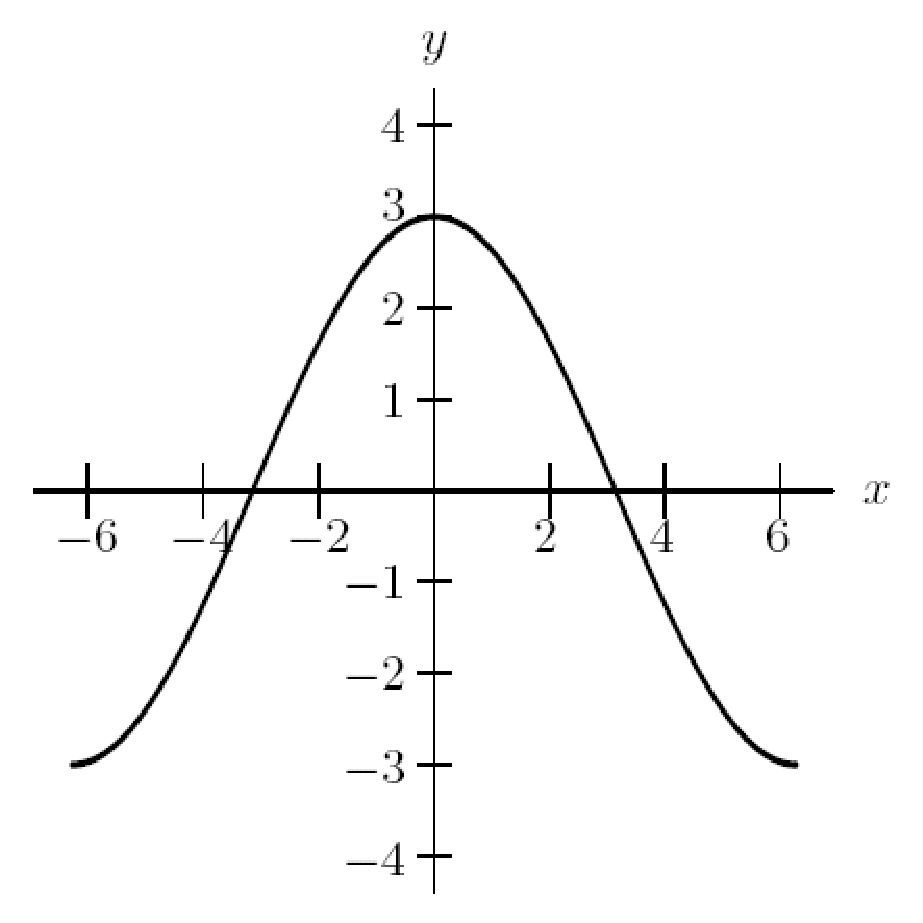
\includegraphics{SVC.01.05.030.ps}}

\begin{minipage}{0.4\columnwidth}
    \begin{enumerate}
        \item $y = 3 \cos(2x)$
        \item $y = 3 \cos(x/2)$
        \item $y = 3 \sin(2x)$
        \item $y = 3 \sin(x/2)$
    \end{enumerate}
\end{minipage}
\begin{minipage}{0.6\columnwidth}
    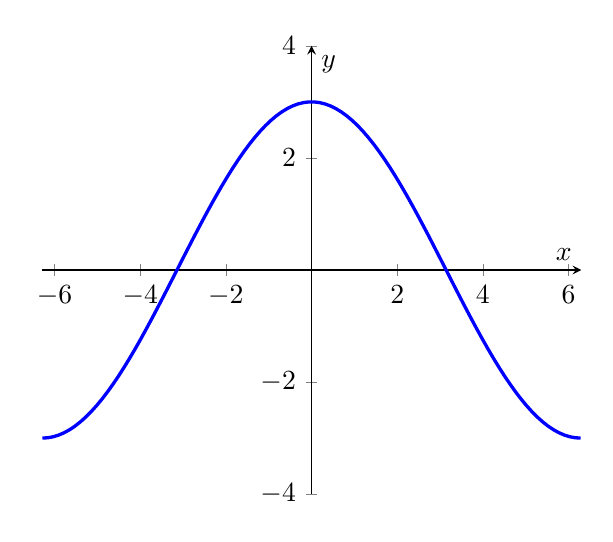
\begin{tikzpicture}
        \begin{axis}[axis lines=center, xlabel={$x$}, ylabel={$y$}, xmin=-6.3, xmax=6.3,
                ymin=-4, ymax=4]
                \addplot[color=blue, very thick,domain=-2*pi:2*pi, samples=100]
                {3*cos(0.5*deg(x))+0};
            \end{axis}
    \end{tikzpicture}
\end{minipage}

% ConcepTests - to accompany Calculus 4th Edition, Hughes-Hallet et al. John Wiley \& Sons.
